%-----------------------------------------------------------------------
% Installation : M2eclipse
% 
%-----------------------------------------------------------------------
%\newpage

%-----------------------------------------------------------------------
\section{Configuration}
Pour pouvoir utiliser toutes les fonctionalités de Maven sous Eclipse, deux étapes de configuration sont nécessaires.

\subsection{Configuration d'Eclipse}
Il faut configurer Eclipse pour s'exécuter avec un JDK et non un JRE sinon ce message d'erreur pourrait s'afficher : 

\begin{center}
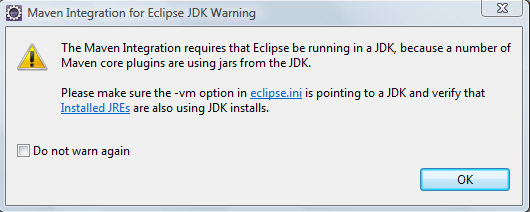
\includegraphics[width=0.4\linewidth]{../../resources/images/guide_installation/warningJRE.png}
\end{center}

\noindent
Pour ce faire, il faut éditer le fichier \emph{eclipse.ini} situé à la racine du répertoire d'Eclipse. Rajoutez les lignes suivantes au début du fichier~:\\

\smallskip 

\begin{tabular}[!t]{l|l}
sous Linux&sous Windows\\
\verb|-vm|&\verb|-vm|\\
\verb|<jdkXXXX>/bin/java|&\verb|<jdkXXXX>\bin\javaw.exe|\\
\end{tabular}\\

\medskip 
\noindent
Où \verb|<jdkXXX>| désigne le répertoire du jdk que vous voulez utiliser, par exemple \\
\verb|c:\MesProgrammes\java\java_EE_5_SDK_Update_7\SDK\jdk|
(pour conna\^itre la valeur par défaut, vous pouvez regarder la valeur de la variable d'environnement JAVA\_HOME).

\medskip 
\begin{center}
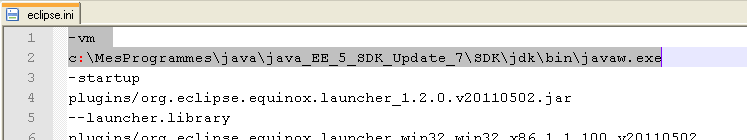
\includegraphics[width=1.0\linewidth]{../../resources/images/guide_installation/eclipse_ini.png}
\end{center}

\medskip 
\noindent
N'ESSAYEZ PAS d'utiliser \%JAVA\_HOME\% dans le eclipse.ini, ce n'est pas pris en charge.


%----------------------------------------------------------------------------------------------------------
\subsection{Configuration de Maven}
Si vous \^etes derrière un proxy, la dernière étape consiste à configurer Maven pour utiliser le proxy. Pour ce, il faut ajouter un fichier \emph{settings.xml} dans la racine de Maven. Ce répertoire est situé à l'endroit suivant~:\\

\smallskip 

\begin{tabular}[!t]{ll}
sous Linux&\verb|~/.m2|\\
sous Windows&\verb|C:\Documents and Settings\%USER%\.m2|
\end{tabular}\\

\bigskip 

\noindent
Voici un exemple de fichier settings que vous pouvez utiliser à l'IGN~:
\begin{scriptsize}
\begin{verbatim}
<settings xmlns="http://maven.apache.org/SETTINGS/1.0.0"
  xmlns:xsi="http://www.w3.org/2001/XMLSchema-instance"
  xsi:schemaLocation="http://maven.apache.org/SETTINGS/1.0.0
                      http://maven.apache.org/xsd/settings-1.0.0.xsd">
  <interactiveMode>true</interactiveMode>
  <usePluginRegistry>false</usePluginRegistry>
  <offline>false</offline>
  <proxies>
    <proxy>
      <active>true</active>
      <port>3128</port>
      <host>proxy.ign.fr</host>
      <nonProxyHosts>localhost</nonProxyHosts>
    </proxy>
  </proxies>
  <profiles>
    <profile>
      <id>cogit</id>
      <activation>
        <activeByDefault>true</activeByDefault>
      </activation>
      <repositories>
        <repository>
          <id>central</id>
          <name>Central Maven Repository</name>
          <url>http://repo2.maven.org/maven2</url>
        </repository>
        <repository>
          <id>releases</id>
          <name>Nexus Releases Repository</name>
          <url>https://dionysos2.ign.fr/nexus-webapp-1.4.1/content/repositories/releases/</url>
        </repository>
      </repositories>
    </profile>
  </profiles>
  <activeProfiles>
    <activeProfile>cogit</activeProfile>
  </activeProfiles>
</settings>
\end{verbatim}
\end{scriptsize}




